\chapter{\babEmpat}

\section{Implementasi Pengujian Autentikasi}

\section{Implementasi Pengujian Performa}

\section{Implementasi Integrasi VxLang}

\section{Analisis Pengujian Autentikasi  VxLang}
\subsection{Analisis Statis}
\subsection{Analisis Dinamis}

\section{Analisis Performa \f{Overhead} VxLang}
Hasil dari percobaan performa overhead dan perubahan ukuran file setelah penerapan virtualisasi kode menggunakan VxLang. Percobaan ini dilakukan pada algoritma Quick Sort dan enkripsi AES-CBC-256.

\subsection{Hasil Pengujian Performa \f{Quick Sort}}
Tabel \ref{tab:quick_sort_performance} menyajikan hasil pengukuran waktu rata-rata dan standar deviasi dari algoritma Quick Sort yang dijalankan sebanyak 100 kali untuk setiap ukuran array, baik sebelum maupun sesudah virtualisasi menggunakan VxLang.

\begin{table}[htbp]
    \centering
    \caption{Hasil Pengujian Waktu Eksekusi Quick Sort (ms)}
    \label{tab:quick_sort_performance}
    \begin{tabularx}{\textwidth}{@{}|X|X|X|X|X|@{}}
    \hline
        \multirow{2}{*}{\textbf{Ukuran Array}} & \multicolumn{2}{c|}{\textbf{Tanpa Virtualisasi}} & \multicolumn{2}{c|}{\textbf{Virtualisasi}}\\
        \cline{2-5}
        & \textbf{Rata-rata Waktu (ms)} & \textbf{Standar Deviasi (ms)} & \textbf{Rata-rata Waktu (ms)} & \textbf{Standar Deviasi (ms)}\\
        \hline
        100                     & 0.01 & 0.00 & 5.15 & 0.42 \\
        \hline
        1000                    & 0.09 & 0.00 & 53.08 & 5.52 \\
        \hline
        5000                    & 0.61 & 0.09 & 300.64 & 26.13 \\
        \hline
        10000                   & 1.38 & 0.22 & 585.70 & 79.88 \\
        \hline
        50000                   & 8.45 & 0.73 & 3,434.32 & 592.92 \\
        \hline
        100000                  & 17.86 & 1.42 & 6,771.09 & 553.09 \\
        \hline
        500000                  & 106.16 & 5.61 & 29,698.73 & 3,518.63 \\
        \hline
        1000000                 & 216.59 & 9.49 & 45,186.90 & 6,198.38 \\
        \hline
    \end{tabularx}
\end{table}

\begin{figure}[htbp]
    \centering
    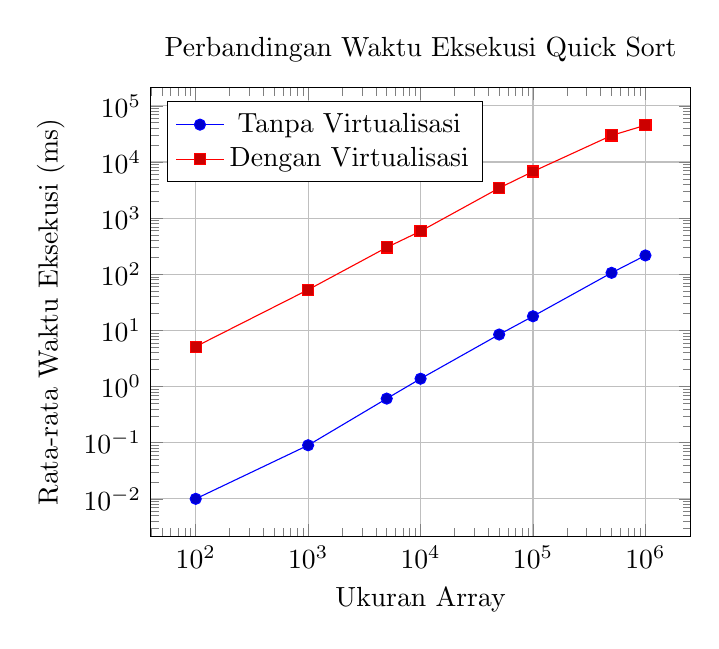
\begin{tikzpicture}
        \begin{axis}[
            xlabel={Ukuran Array},
            ylabel={Rata-rata Waktu Eksekusi (ms)},
            xmode=log,
            log basis x={10},
            ymode=log,
            log basis y={10},
            legend pos=north west,
            title={Perbandingan Waktu Eksekusi Quick Sort},
            grid=major,
        ]
        \addplot coordinates {
            (100, 0.01)
            (1000, 0.09)
            (5000, 0.61)
            (10000, 1.38)
            (50000, 8.45)
            (100000, 17.86)
            (500000, 106.16)
            (1000000, 216.59)
        };
        \addlegendentry{Tanpa Virtualisasi};

        \addplot coordinates {
            (100, 5.15)
            (1000, 53.08)
            (5000, 300.64)
            (10000, 585.70)
            (50000, 3434.32)
            (100000, 6771.09)
            (500000, 29698.73)
            (1000000, 45186.90)
        };
        \addlegendentry{Dengan Virtualisasi};
        \end{axis}
    \end{tikzpicture}
    \caption{Perbandingan Waktu Eksekusi Algoritma Quick Sort antara Versi Tanpa dan Dengan Virtualisasi VxLang.}
    \label{fig:quick_sort_performance}
\end{figure}

Berdasarkan Tabel \ref{tab:quick_sort_performance} ,terlihat adanya peningkatan waktu eksekusi yang signifikan pada algoritma Quick Sort setelah divirtualisasi menggunakan VxLang. Peningkatan ini terlihat semakin besar seiring dengan bertambahnya ukuran array. Sebagai contoh, untuk array berukuran 100, waktu eksekusi rata-rata meningkat dari 0.01 ms menjadi 5.15 ms, yang menunjukkan overhead sekitar 51400\%. Untuk array yang lebih besar seperti 1.000.000 elemen, waktu eksekusi meningkat dari 216.59 ms menjadi 45186.90 ms, dengan overhead sekitar 20860\%. Peningkatan standar deviasi juga menunjukkan bahwa waktu eksekusi menjadi lebih bervariasi setelah virtualisasi. Hal ini mengindikasikan adanya overhead yang substansial yang diperkenalkan oleh mesin virtual VxLang dalam mengeksekusi instruksi virtual dibandingkan dengan eksekusi kode native.

\subsection{Hasil Pengujian Performa Enkripsi AES-CBC-256}
Tabel \ref{tab:aes_performance} menyajikan hasil benchmarking enkripsi AES-CBC-256 dengan 1.000.000 blok data, di mana setiap blok berukuran 1024 bytes, sebelum dan sesudah virtualisasi menggunakan VxLang.

\begin{table}[htbp]
  \centering
  \caption{Hasil Pengujian Performa Enkripsi AES-CBC-256}
  \label{tab:aes_performance}
  \begin{tabular}{|l|c|c|}
    \hline
    \bo{Metrik}                                     & \bo{Tanpa Virtualisasi} & \bo{Virtualisasi} \\
    \hline
    Total Waktu Enkripsi (ms)                  & 2,722.96            & 13,193.51            \\
    \hline
    Total Waktu Dekripsi (ms)                  & 2,055.01            & 12,529.90            \\
    \hline
    Rata-rata Waktu per Blok Enkripsi (ms)     & 0.00272            & 0.01319             \\
    \hline
    Rata-rata Waktu per Blok Dekripsi (ms)     & 0.00206            & 0.01253             \\
    \hline
    \textit{Throughput} Enkripsi (MB/s)               & 358.64             & 74.02               \\
    \hline
    \textit{Throughput} Dekripsi (MB/s)               & 475.21             & 77.94               \\
    \hline
    \textit{Throughput} Gabungan (MB/s)               & 416.92             & 75.98               \\
    \hline
  \end{tabular}
\end{table}

Hasil pengujian enkripsi AES-CBC-256 menunjukkan overhead performa yang signifikan setelah penerapan VxLang. Total waktu enkripsi meningkat dari 2,722.96 ms menjadi 13,193.51 ms, yang merupakan peningkatan sekitar 384\%. Total waktu dekripsi juga mengalami peningkatan yang serupa, dari 2,055.01 ms menjadi 12,529.90 ms (sekitar 510\%). Peningkatan ini juga tercermin pada penurunan throughput (kecepatan pemrosesan data). Throughput enkripsi menurun dari 358.64 MB/s menjadi 74.02 MB/s, dan throughput dekripsi menurun dari 475.21 MB/s menjadi 77.94 MB/s. Penurunan throughput gabungan juga signifikan, dari 416.92 MB/s menjadi 75.98 MB/s. Hasil ini mengkonfirmasi bahwa virtualisasi kode dengan VxLang memperkenalkan overhead yang cukup besar pada operasi komputasi intensif seperti enkripsi.

\subsection{Hasil Pengujian Ukuran File}
Tabel \ref{tab:file_size} menyajikan ukuran file executable (dalam KB) untuk berbagai program sebelum dan sesudah virtualisasi menggunakan VxLang.

\begin{table}[htbp]
  \centering
  \caption{Hasil Pengujian Ukuran File (KB)}
  \label{tab:file_size}
  \begin{tabular}{@{}|l|c|c|@{}}
    \hline
    \multirow{2}{*}{\textbf{Program}} & \multicolumn{2}{c|}{\textbf{Ukuran File}} \\
    \cline{2-3} & \bo{Tanpa Virtualisasi} & \bo{Virtualiasi} \\
    \hline
    quick\_sort  & 119                                  & 1,951                               \\
    \hline
    encryption   & 131                                  & 1,834                               \\
    \hline
    size         & 97,802                               & 112,716                             \\
    \hline
    console      & 105                                  & 1,942                               \\
    \hline
    app\_imgui   & 1,773                                & 2,753                               \\
    \hline
    app\_qt      & 145                                  & 1,954                               \\
    \hline
  \end{tabular}
\end{table}

Hasil pengukuran ukuran file menunjukkan bahwa penerapan virtualisasi kode menggunakan VxLang secara umum meningkatkan ukuran file executable. Peningkatan ukuran file sangat signifikan untuk program-program kecil seperti quick\_sort, encryption, dan console, di mana ukurannya meningkat lebih dari sepuluh kali lipat. Untuk aplikasi GUI yang lebih besar seperti app\_imgui dan app\_qt, peningkatan ukuran file juga terlihat, meskipun persentasenya mungkin lebih kecil dibandingkan dengan program yang lebih kecil. Peningkatan ukuran file size relatif lebih kecil, namun tetap signifikan. Peningkatan ukuran ini kemungkinan disebabkan oleh penambahan interpreter mesin virtual VxLang dan bytecode yang dihasilkan ke dalam executable yang dilindungi.
